\documentclass[10pt,conference,compsocconf]{IEEEtran}

\usepackage{hyperref}
\usepackage{graphicx}	% For figure environment
\usepackage{amsmath}
\usepackage{placeins}

\begin{document}
\title{\vspace*{-2em}NX414 - Mini-project Report\vspace*{-1.8em}}

\author{
  Kolly Florian, Mikami Sarah, Montlahuc Louise \\
  Team 1
}

\maketitle

\begin{abstract}
    This report presents our approach to predicting neural activity from IT neurons given visual stimuli. We explore various models, ranging from simple regression on pixel data to more sophisticated task- and data-driven neural network models. Our goal is to develop the most accurate model for predicting IT neural activity. By finetuning a pretrained ResNeXt-50 model on the neural data, we obtain a final \(R^2\) score of 0.45.
\end{abstract}

% \section{Data}
% The data used in this project comes from DiCarlo \textit{et al.} (2015) \cite{Majaj2015}, where they recorded neural activity from the inferior temporal (IT) cortex from non-human primates while showing them images. The data consists of the stimuli images and the corresponding average firing rate (from 70 to 170 ms) per each 168 recorded IT neurons.

\section{Regression on stimuli}
Before trying complex models, we analysed the possibility of predicting neural activity directly from pixels. BLABLA. The results are presented in Table \ref{table:regression}.

\begin{table}[h!]
    \centering
    \begin{tabular}{|l|c|c|c|}
        \hline
        Regression & Param. & \(R^2\) on train & \(R^2\) on valid. \\
        \hline
        Linear & - & 0.355 & -0.037 \\
        Linear & PCA & ? & ? \\
        Ridge & \(\alpha=1\) & 0.999 & -1.167 \\
        Ridge & PCA, \(\alpha=1\) & ? & ? \\
        \hline
    \end{tabular}
    \caption{Results when doing regression on the stimuli (pixels)}
    \label{table:regression}
\end{table}
\vspace{-1.5em}

We observe that there is a clear overfitting of these methods on the training data, leading to an overall bad generalisation and hence bad scores on the validation set.

\section{Regression on pretrained networks}
To obtain better scores, we then try to predict the neural activity with a task-driven modeling approach. The hypothesis is that training a network to perform relevant behavioral task makes it learn representations that resemble those of the brain. Our selection of models is inspired by the leaderboard of Brain-Score \cite{SchrimpfKubilius2018BrainScore, Schrimpf2020integrative}. We chose six models, including some of the best performing ones, also taking into account the limited compute ressources at disposal: ResNet-18, ResNet-50 \cite{ResNet}, ConvNeXt (base) \cite{ConvNeXt}, ViT (base) \cite{ViT}, ResNeXt-50 \cite{ResNeXt} and DinoV2 \cite{DinoV2}\footnote{Thanks to the teaching team for this recommandation}.

For each model, we select the last three layers and save the activations when we pass the images through the model. We perform three types of probing on the activations in order to predict the IT neural activity: a simple linear regression, a ridge regression and a two-layers MLP. Table \ref{table:pretrained} lists the best \(R^2\) score on the validation data per model, indicating which layer and probing method yield this score.

\begin{table}[h!]
    \centering
    \begin{tabular}{|l|c|c|c|}
        \hline
        Model & Layer & Probing & \(R^2\) \\
        \hline
        ResNet-18 & layer3 & Ridge & 0.269 \\
        ResNet-50 & layer3 & Ridge & 0.369 \\
        ResNeXt & layer3 & Ridge & 0.391 \\
        ConvNeXt & layer7 & Ridge & 0.199 \\
        ViT & encoder & Ridge & 0.306 \\
        DinoV2 & ? & ? & ? \\
        \hline
    \end{tabular}
    \caption{Best result of probing pretrained layers}
    \label{table:pretrained}
\end{table}

The decision of selecting the last three layers of each model was made after an analysis of the distribution of the explained variance per neuron with respect to the layer of a pretrained ResNet-50 network. Figure \ref{fig:explvar} clearly shows that the explained variance distribution improves as the depth of the model increases.

\begin{figure}[h!]
    \centering
    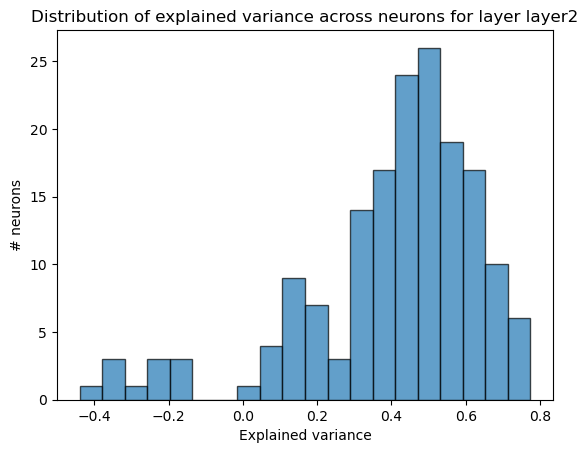
\includegraphics[width=0.8\columnwidth]{explvar.png}
    \caption{Distribution of explained variance across ResNet-50 depth}
    \label{fig:explvar}
\end{figure}
\FloatBarrier

\section{Finetuning pretrained models}
The previous results indicate that ResNet-50 and ResNeXt are good candidates for finding the best model. Taking these models as backbone, we finetune them either I) a task-driven task (classify objects in images) or II) a data-driven task (regress neural activity given images). Specifically, we cut the network after a given layer and add either a classification or regression head. After experimenting with various training scheme and heads, we found our best result with an \(R^2\) score of 0.45 using a data-driven approach. The backbone is given by ResNeXt-50 cut before layer 4, with a two-layers MLP preceded by an adaptive average pooling \cite{AdaptiveAvgPool}. The training scheme consists of 30 epochs with a linear learning rate warmup during the first 5 epochs up to \(10^{-6}\) followed by a cosine annealing scheduler down to 0.

\newpage
\bibliographystyle{IEEEtran}
\bibliography{literature}

\end{document}